\doublespacing % Do not change - required

\chapter{Methods \& Experimental Setup}
\label{ch2}

%%%%%%%%%%%%%%%%%%%%%%%%%%%%%%%%%%%%%%%
% IMPORTANT
\begin{spacing}{1} %THESE FOUR
\minitoc % LINES MUST APPEAR IN
\end{spacing} % EVERY
\thesisspacing % CHAPTER
% COPY THEM IN ANY NEW CHAPTER
%%%%%%%%%%%%%%%%%%%%%%%%%%%%%%%%%%%%%%%

\subsection{Formal Problem Definition: A Two-Stage Approach to Explainable Recommendation}

\subsubsection{AGENTIC Cold-Start Pipeline}



\begin{figure}[h!]
\centering
\begin{tikzpicture}[
node distance=1cm,
stage/.style={rectangle, draw, fill=gray!10, text centered, minimum height=3.5cm, minimum width=10cm},
icon/.style={font=\Huge, inner sep=0pt, text=black},
label/.style={font=\bfseries, text=black},
arrow/.style={-Stealth, thick, draw=blue!60}
]

% STAGE 1
\node (stage1) [stage] {};
\node at (stage1.north) [label, yshift=-0.5cm] {1. Automated Feature Engineering};
\node (raw_data) at ([xshift=-3cm]stage1.center) {Raw Data};
\node (features) [icon] at ([xshift=3cm]stage1.center) {\faProjectDiagram};
\node[below=0.5cm of features] {Engineered Features};
\draw [arrow] (raw_data) -- (features);

% STAGE 2
\node (stage2) [stage, below=of stage1, yshift=-1.5cm] {};
\node at (stage2.north) [label, yshift=-0.5cm] {2. User Clustering Optimisation};
\node (cluster_a) [icon] at ([xshift=-3cm]stage2.center) {\faUsers};
\node (cluster_b) [icon] at (stage2.center) {\faUsers};
\node (cluster_c) [icon] at ([xshift=3cm]stage2.center) {\faUsers};
\node[below=0.2cm of cluster_b, text width=5cm, align=center] {User Clusters Minimising Intra-Cluster RMSE};


% STAGE 3
\node (stage3) [stage, below=of stage2, yshift=-1.5cm] {};
\node at (stage3.north) [label, yshift=-0.5cm] {3. Cold-Start User Assignment};
\node (new_user) [icon] at ([xshift=-4cm]stage3.center) {\faUserPlus};
\node[below=0.1cm of new_user] {New User};
\node (bayes_q) [icon] at (stage3.center) {\faComments};
\node[below=0.1cm of bayes_q] {Bayesian Questioning};
\node (assigned) [icon] at ([xshift=4cm]stage3.center) {\faUserCheck};
\node[below=0.1cm of assigned] {User is assigned to a cluster};
\draw [arrow, dashed] (new_user) -- (bayes_q);
\draw [arrow, dashed] (bayes_q) -- (assigned);

% Main connecting arrows
\draw [arrow, ultra thick] (features) -- (stage2.north);
\draw [arrow, ultra thick] (stage2.south) -- (new_user);
\end{tikzpicture}
\caption{Proposal for a three-stage workflow for recommendation. \textbf{1) Automated Feature Engineering:} Raw data is transformed into an engineered feature space. \textbf{2) User Clustering:} Users are grouped into distinct preference clusters. \textbf{3) Cold-Start User Assignment:} A new user is assigned to a cluster via an iterative Bayesian questioning process.}
\label{fig:fixed_workflow}
\end{figure}



The AGENTIC framework addresses the cold-start problem through two sequential stages: (1) \textbf{Feature Engineering and Clustering} -- automatically discovering interpretable feature representations that enable both accurate recommendations and meaningful user clustering, and (2) \textbf{Bayesian User Profiling} -- efficiently assigning new users to clusters through strategic questioning. While this thesis focuses exclusively on Stage 1, we present the complete framework to establish the broader research context and motivation.

\subsection*{Stage 1: Optimal Feature Representation Learning}


Let the dataset be $\mathcal{D} = \{(u_i, v_j, r_{ij}, \mathbf{s}_{ij})\}$, where $u_i$ denotes users, $v_j$ denotes items, $r_{ij}$ represents the primary user-item interaction strength, and $\mathbf{s}_{ij}$ is a vector of \textbf{supplementary data} columns (e.g., temporal, contextual, or demographic information).

The core problem is to discover an optimal feature transformation function, $T(\cdot, \theta)$, parameterized by $\theta$. This function selects and transforms a subset of the supplementary data, $\mathbf{s}_{ij}$, to create an engineered feature representation, $\mathbf{f}_{ij} = T(\mathbf{s}_{ij}, \theta)$. These engineered features are then used to augment a baseline matrix factorization model.

The optimization objective is to find the parameters $\theta^*$ that define the feature set that minimizes our objective function, $J(\cdot)$:
\[
    \theta^* = \arg\min_{\theta} J(T(\mathcal{D}_{\text{train}}, \theta))
\]
where the objective function $J(\mathbf{F})$ over a set of engineered feature representations $\mathbf{F}$ is defined as:
\[
    J(\mathbf{F}) = 
    \underbrace{\alpha \cdot \frac{\text{RMSE}_{\text{cluster}}(\mathbf{F})}{\text{RMSE}_{\text{baseline}}}}_{\text{Relative Performance Gain}} - 
    \underbrace{\beta \cdot \text{SilhouetteScore}(\mathbf{F})}_{\text{Cluster Interpretability}}
\]
Here, $\alpha$ and $\beta$ are weighting coefficients. The first term measures recommendation performance as the Root Mean Square Error of the cluster-based models (trained on the baseline interactions + engineered features $\mathbf{F}$) relative to a pure matrix factorization baseline (trained only on baseline interactions). The second term uses the silhouette score to reward the interpretability of the clusters formed from these enhanced user representations.

\subsection*{Stage 2: Bayesian User Profiling (Future Work)}
For new users, efficient cluster assignment is achieved through strategic questioning that maximizes information gain. Let $C$ represent the set of user clusters and $E$ represent evidence from user responses. The optimal questioning strategy sequentially selects questions $Q$ that maximize expected information gain:
\[
    IG(Q) = H(C|E) - \sum_{a \in \mathcal{A}_Q} P(a|E) \cdot H(C|E,a)
\]
This approach enables rapid cold-start profiling by efficiently reducing uncertainty about cluster membership. The questioning system can be trained on synthetic conversational data, as demonstrated by recent surveys on LLMs in recommendation \cite{wu2023survey}, proving the feasibility of using large language models to generate realistic user-system interactions for training conversational recommendation systems.

\subsection*{Scope and Contributions}
This thesis exclusively addresses Stage 1 of the AGENTIC framework, focusing on the automated discovery of optimal feature representations that simultaneously maximize recommendation accuracy and cluster interpretability. The bilevel optimization approach provides a principled foundation for transitioning from latent factor models to explainable user archetypes, enabling the broader vision of conversational recommendation systems while maintaining competitive predictive performance.

The key contribution lies in formalizing feature engineering for explainable recommendation as a multi-objective optimization problem that explicitly balances prediction accuracy, cluster quality, and model complexity, thereby providing a systematic approach to discovering interpretable user representations in recommendation systems.






\subsection{AGENTIC Multi-Agent System for Collaborative Problem-Solving}

    % We load TikZ libraries for positioning, shapes, arrows, and fitting nodes.
    \begin{figure*}[ht!]
    \centering
    % We load TikZ libraries for positioning, shapes, arrows, and fitting nodes.
    \usetikzlibrary{positioning, shapes.geometric, arrows.meta, fit, calc}
    
    \begin{tikzpicture}[
        node distance=1.2cm and 1.8cm,
        agent/.style={rectangle, rounded corners, draw=black, very thick, text centered, align=center, text width=3.5cm, minimum height=2.2cm},
        agent_discovery/.style={agent, fill=blue!10},
        agent_strategy/.style={agent, fill=purple!10},
        agent_generation/.style={agent, fill=green!10},
        main_process/.style={rectangle, rounded corners, draw=black!80, fill=gray!5, inner sep=5pt, text width=3.5cm, minimum height=1.5cm, align=center, font=\bfseries},
        team_box/.style={rectangle, draw=black!50, dashed, inner sep=0.6cm, rounded corners},
        artifact/.style={rectangle, draw=black!70, fill=gray!15, inner sep=5pt, align=center, font=\bfseries},
        flow_arrow/.style={-Latex, very thick, blue!60!black},
        feedback_arrow/.style={-Latex, very thick, orange!80!black, dashed, rounded corners=15pt}
    ]

    % --- Column 1: Phase 1 ---
    \node[main_process] (db) {
\includegraphics[width=0.5cm]{imgs/icon_database.png} \\ Goodreads Dataset};
    
    \node[agent_discovery, below=2cm of db] (representer) {\textbf{DataRepresenter} \\ \small Creates SQL views};
    \node[agent_discovery, below=0.3cm of representer] (quant) {\textbf{QuantitativeAnalyst} \\ \small Runs statistical tests};
    \node[agent_discovery, below=0.3cm of quant] (pattern) {\textbf{PatternSeeker} \\ \small Finds non-obvious correlations};
    \node[team_box, fit=(representer) (quant) (pattern), label={[font=\bfseries]above:
\includegraphics[width=0.7cm]{imgs/icon_chat.png} Phase 1}] (phase1_box) {};

    % --- Column 2: Phase 2 ---
    \node[agent_strategy, right=of representer] (feature_engineer) {\textbf{FeatureEngineer} \\ \small Proposes hypotheses};
    \node[agent_strategy, below=0.3cm of feature_engineer] (strategist) {\textbf{StrategistAgent} \\ \small Critiques for business value};
    \node[agent_strategy, below=0.3cm of strategist] (engineer) {\textbf{EngineerAgent} \\ \small Critiques for feasibility};
    \node[team_box, fit=(feature_engineer) (strategist) (engineer), label={[font=\bfseries]above:
\includegraphics[width=0.7cm]{imgs/icon_chat.png} Phase 2}] (phase2_box) {};

    % --- Column 3: Phase 3 ---
    \node[agent_generation, right=of feature_engineer] (realizer) {\textbf{FeatureRealizer} \\ \small Writes \& validates code via self-correction};
    \node[main_process, below=0.3cm of realizer] (optimizer) {
\includegraphics[width=0.5cm]{imgs/icon_optimization.png} \\ VULCANOptimizer};
    \node[main_process, below=0.3cm of optimizer] (reflection) {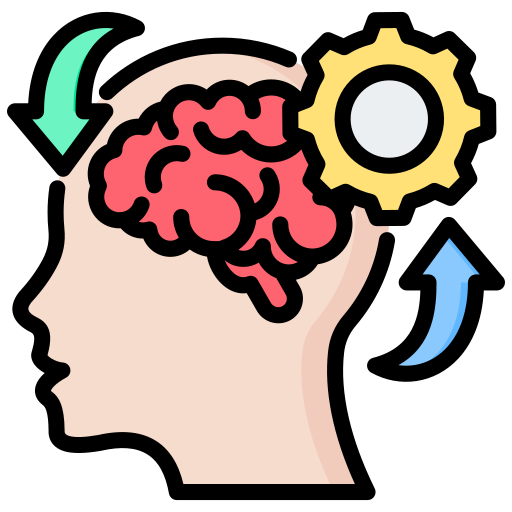
\includegraphics[width=0.5cm]{imgs/icon_reflection.png} \\ Reflection Agent};
    \node[team_box, fit=(realizer) (optimizer) (reflection), label={[font=\bfseries]above:
\includegraphics[width=0.7cm]{imgs/icon_realization.png} Phase 3}] (phase3_box) {};

    % --- Final Output ---
    \node[artifact, fill=green!10, below=1.5cm of phase3_box] (output) {Final Optimized \\ Feature Set};
    
    \draw[flow_arrow] (db) -- ($(phase1_box.north) + (1.5cm, 0)$);    \draw[flow_arrow] (phase1_box) -- node[midway, above] {Insights} (phase2_box);
    \draw[flow_arrow] (phase2_box) -- node[midway, above] {Hypotheses} (phase3_box);
    \draw[flow_arrow] (phase3_box) -- (output);
    
    % The Meta-Learning Feedback Loop (Goes all the way around)
\draw[feedback_arrow] 
    (reflection.south) 
    -- ++(0, -3cm) 
    -| ($(phase1_box.west) - (0.5cm, 0.1cm)$)
    node[pos=0.25, below] {\textbf{Next Epoch}}
    -- (phase1_box.west);

    \end{tikzpicture}
    \caption{The collaborative architecture of the VULCAN system. The process flows from left to right. Phase 1 (Discovery) and Phase 2 (Strategy) involve collaborative `GroupChat` sessions to produce vetted hypotheses. In Phase 3, these are converted into validated code and optimized. The `ReflectionAgent` analyzes the run's performance, creating a meta-learning loop for subsequent epochs.}
    \label{fig:vulcan_architecture_final}
\end{figure*}

Automated feature engineering requires integrating diverse analytical perspectives. We posit that the most effective solution is not a monolithic algorithm but a collaborative multi-agent system that models the workflow of a human data science team. By decomposing the process into specialized roles and enabling structured communication, we can leverage complementary analytical strengths. The AGENTIC system implements this philosophy using Microsoft's AutoGen library, which provides robust capabilities for orchestrating structured conversations between LLM-powered agents.

\begin{table}[h]
\centering
\caption{AGENTIC Agent Roles and Responsibilities}
\label{tab:agent_roles}
\begin{tabular}{|l|l|p{8cm}|}
\hline
\textbf{Team} & \textbf{Agent} & \textbf{Primary Responsibilities} \\
\hline
\multirow{3}{*}{Discovery} & DataRepresenter & Schema analysis, data structure understanding, relationship identification \\
\cline{2-3}
& QuantitativeAnalyst & Statistical analysis, correlation discovery, distribution characterization \\
\cline{2-3}
& PatternSeeker & Trend identification, anomaly detection, temporal pattern analysis \\
\hline
\multirow{3}{*}{Strategy} & HypothesisAgent & Generate testable feature hypotheses from discovered insights \\
\cline{2-3}
& StrategistAgent & Evaluate feasibility, impact assessment, strategic prioritization \\
\cline{2-3}
& EngineerAgent & Implementation complexity analysis, technical feasibility assessment \\
\hline
\end{tabular}
\end{table}

\subsection{Phase 1: Collaborative Discovery and Strategy}

\subsubsection{Discovery Team}

The Discovery Team performs a comprehensive exploratory data analysis (EDA). The \texttt{DataRepresenter} analyzes data structures and schemas, the \texttt{QuantitativeAnalyst} performs statistical tests to find correlations, and the \texttt{PatternSeeker} identifies temporal and behavioral trends. The team collaborates in a \texttt{GroupChat} until a sufficient number of high-quality, structured insights are generated, ensuring a thorough yet efficient exploration.

\subsubsection{Strategy Team}

The Strategy Team transforms the raw insights into concrete feature engineering hypotheses. The \texttt{HypothesisAgent} generates testable ideas from the insights. These are then critiqued in a structured, adversarial discussion by the \texttt{StrategistAgent} for business value and the \texttt{EngineerAgent} for technical feasibility. This collaborative refinement ensures only high-quality, implementable hypotheses proceed to the next phase, outputting a prioritized list of feature specifications.


% FIGURE SUGGESTION: Discovery and Strategy Team workflow diagram
% Caption: Figure 2: Workflow of the Discovery and Strategy Teams in AGENTIC. The Discovery Team conducts multi-perspective EDA through specialized agents, generating structured insights. The Strategy Team then transforms these insights into implementable feature hypotheses through collaborative evaluation and refinement.

\subsection{Phase 2: Feature Realization and Optimization}

This phase transforms the vetted hypotheses from the Strategy Team into an optimized set of features. The process involves two tightly integrated components: \texttt{FeatureRealizer}, which generates and validates code, and \texttt{VULCANOptimizer}, which implements a bilevel optimization framework to find the best-performing feature configurations. The entire workflow is detailed in Table \ref{tab:phase2_details}.

\begin{table*}[ht!]
\centering
\caption{AGENTIC Phase 2: Feature Realization and Optimization Workflow}
\label{tab:phase2_details}
\resizebox{\textwidth}{!}{%
\begin{tabular}{|l|p{11.5cm}|}
\hline
\textbf{Component} & \textbf{Description \& Formalism} \\
\hline
\hline
\multicolumn{2}{|c|}{\textbf{Feature Realization Process}} \\
\hline
\textbf{Agent} & \textbf{FeatureRealizer}: An LLM agent responsible for code generation. \\
\hline
\textbf{Process} & 
\begin{enumerate}[label=\arabic*), noitemsep, topsep=0pt]
    \item \textbf{Generate}: Translates a feature hypothesis into a parameterized Python function.
    \item \textbf{Validate}: Executes the generated code in a secure sandbox to verify syntactic and runtime correctness against test data.
    \item \textbf{Self-Correct}: If validation fails, the error traceback is fed back to the agent for iterative refinement (max 3 attempts).
    \item \textbf{Register}: Successfully validated functions are added to a feature registry, making them available to the optimizer.
\end{enumerate} \\
\hline
\hline
\multicolumn{2}{|c|}{\textbf{Bilevel Optimization Framework (VULCANOptimizer)}} \\
\hline
\textbf{Outer Loop} & 
\textbf{Method}: Bayesian Optimization using a Tree-structured Parzen Estimator (TPE) to efficiently search the hyperparameter space $\Theta$. \\
\textbf{Objective}: Find the optimal parameter set $\theta^*$ that maximizes a reward function $J(\theta)$.
\begin{align*}
    \theta^* = \arg\max_{\theta \in \Theta} J(\theta)
\end{align*}
\\
\hline
\textbf{Inner Loop} & 
\textbf{Method}: k-fold Cross-Validation to provide a robust evaluation of $J(\theta)$ for a given trial configuration $\theta$. \\
\textbf{Model}: Employs LightFM factorization machines to model user-item interactions using the generated features. \\
\hline
\end{tabular}%
}
\end{table*}

\subsubsection{Bilevel Optimization via Bayesian Optimization}

The core of the \texttt{VULCANOptimizer} is a bilevel optimization framework. The inner loop evaluates feature quality, while the outer loop performs a guided search for the optimal feature hyperparameters, $\theta^*$. Given the high dimensionality of the search space $\Theta$ and the absence of gradient information for our objective function $J(\theta)$, we employ Bayesian Optimization (BO).

The motivation for BO extends beyond merely handling a costly objective function; it is chosen for its efficiency in navigating complex, high-dimensional parameter spaces. Unlike grid search or random search, BO intelligently uses the results of past evaluations to inform which set of parameters to try next. This is achieved by building and updating a probabilistic surrogate model of the objective function. The process operates in an iterative loop. First, a Tree-structured Parzen Estimator (TPE) models two separate probability distributions: $l(\theta)$ for the parameters associated with the best objective scores observed, and $g(\theta)$ for all other parameters. The next set of parameters to evaluate, $\theta_{next}$, is chosen by optimizing an acquisition function based on Expected Improvement (EI), which is maximized by sampling points where the ratio $l(\theta)/g(\theta)$ is high. This strategy balances exploitation (sampling near known good results) and exploration (sampling in uncertain regions). The objective function $J(\theta_{next})$ is then evaluated, and the new result $(\theta_{next}, J(\theta_{next}))$ is used to update the TPE distributions. This loop continues until a predefined amount of trials is exhausted, with the final output being the parameter set $\theta^*$ that yielded the highest score.

\section{Experimental Setup}
\label{sec:experimental-setup}

We use the Goodreads Fantasy dataset, which has the most reviews and user-item interactions among available genres. Only users and books with at least one rating are included. Table~\ref{tab:dataset-stats} summarizes the dataset.

\begin{table}[h]
\centering
\caption{Key dataset statistics.}
\label{tab:dataset-stats}
\begin{tabular}{ll}
\toprule
Statistic & Value \\
\midrule
Number of users & 256,088 \\
Number of books & 258,585 \\
Number of ratings & 3,424,641 \\
Average ratings per user & 13.37 \\
Average ratings per book & 13.24 \\
Rating scale & 1--5 \\
Mean rating & 3.82 \\
\bottomrule
\end{tabular}
\end{table}

\subsection{Cross-Validation}

We use 5-fold cross-validation, stratified by user activity: each user's ratings are spread as evenly as possible across folds. This ensures all users appear in both train and test splits.

\begin{table}[h]
\centering
\caption{Cross-validation protocol.}
\begin{tabular}{ll}
\toprule
Parameter & Setting \\
\midrule
Folds & 5 \\
Stratification & By user activity \\
Split logic & User ratings distributed evenly \\
\bottomrule
\end{tabular}
\end{table}

\subsection{Baselines}

Table~\ref{tab:baselines} lists the baseline models used for comparison.

\begin{table}[h]
\centering
\caption{Evaluated baseline models.}
\label{tab:baselines}
\begin{tabular}{ll}
\toprule
Model & Description \\
\midrule
LightFM & Hybrid matrix factorization \\
SVD (Surprise) & Matrix factorization (explicit) \\
Random Forest & Regression on numeric features \\
Popularity & Most popular books \\
Featuretools & Automated feature engineering \\
\bottomrule
\end{tabular}
\end{table}

\subsection{Evaluation Metrics}

Performance is measured by RMSE, MAE, NDCG@k, Precision@k, and Recall@k. Table~\ref{tab:metrics} gives a summary.

\begin{table}[h]
\centering
\caption{Evaluation metrics.}
\label{tab:metrics}
\begin{tabular}{ll}
\toprule
Metric & Description \\
\midrule
RMSE & Root Mean Squared Error \\
MAE & Mean Absolute Error \\
NDCG@k & Normalized Discounted Cumulative Gain ($k=5,10,20$) \\
Precision@k & Relevant items in top-$k$ \\
Recall@k & Relevant items retrieved in top-$k$ \\
\bottomrule
\end{tabular}
\end{table}

\paragraph{NDCG Definition.}
For a ranked list of $k$ items, NDCG@k is:
\[
\mathrm{NDCG}@k = \frac{1}{\mathrm{IDCG}@k} \sum_{i=1}^k \frac{2^{\mathrm{rel}_i} - 1}{\log_2(i+1)}
\]
where $\mathrm{rel}_i$ is the relevance of the item at rank $i$, and $\mathrm{IDCG}@k$ is the maximum possible DCG for the ground truth.

\textit{Note:} All metrics are averaged across the 5 CV folds. NDCG and ranking metrics are only computed for models that output ranked lists.


%CV Folds
% Dataset statistics 
% BO Detail 


% FIGURE SUGGESTION: System architecture diagram
% Caption: Figure 3: Complete AGENTIC system architecture showing the flow from raw data through Discovery and Strategy Teams to feature realization and bilevel optimization. The diagram illustrates the multi-agent collaboration, self-correction loops, and integration with the optimization framework.

% FIGURE SUGGESTION: Bilevel optimization visualization
% Caption: Figure 4: Visualization of the bilevel optimization process in AGENTIC. The outer loop (Bayesian optimization) explores the hyperparameter space of realized features, while the inner loop (cross-validation with LightFM) evaluates each configuration. The multi-objective function balances recommendation quality, cluster interpretability, and feature complexity.